\subsection{Judge}\label{sec:judge}

\subsubsection{Role in the Pipeline}\label{sec:judge-role}

Building upon the LLM-as-a-judge paradigm introduced in \cref{sec:pipeline-justification}, this section explains the judge's operational role within the pipeline. As the judge operates directly on unlabelled production queries, it builds up a golden dataset over time and removes the need to construct and maintain a synthetic test set for evaluation. Furthermore, it produces a structured failure analysis that would otherwise demand a manual root-cause analysis.

As described in \cref{sec:router}, the router produces a full candidate ranking over all eight agents, from which the second-best candidate can be identified. In the live environment, the selected agent directly returns a response to the user. The judge is given the response of the selected agent and a counterfactual response generated by calling the second-ranked candidate with the same query and produces a verdict with justification explaining which one better resolves it. Depending on which stage of the router made the routing decision, this verdict is either written directly into the example store for Stage 1 or passed on to the optimizer. The detailed mechanism behind this distinction is described in \cref{sec:judge-implementation}. \Cref{fig:judge-role} illustrates the general flow.

\begin{figure}
\centering
\pandocbounded{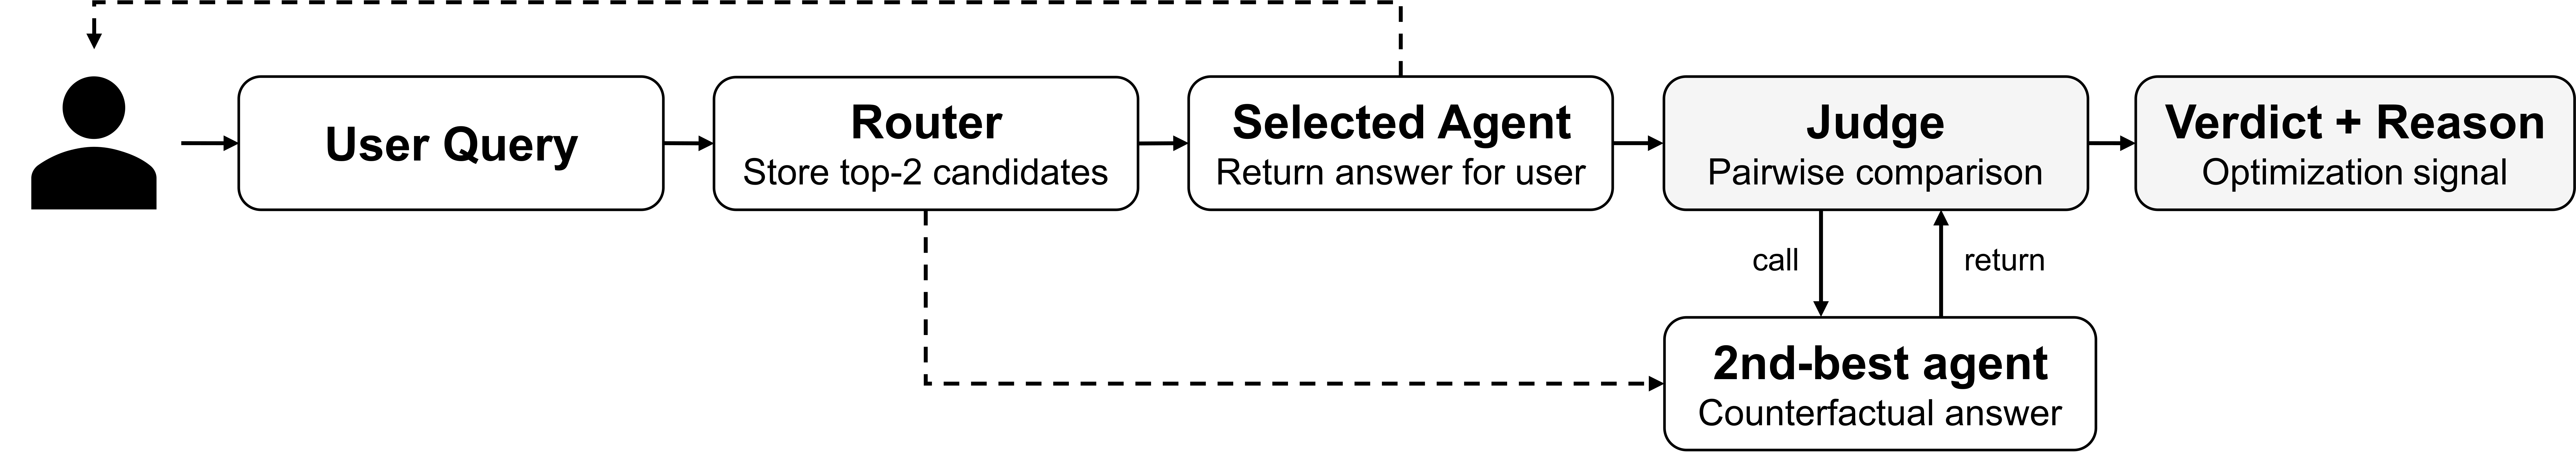
\includegraphics[keepaspectratio]{assets/pipeline/judge-role.png}}
\caption{Role of the judge component within the pipeline.}
\label{fig:judge-role}
\end{figure}


The comparison is restricted to the top two candidates rather than all eight agents. This is a practical decision grounded in empirical observation. The score margin between the second- and third-ranked agent is typically larger than between the first- and second-ranked one, so routing ambiguity is almost always a decision between the top two agents. Restricting the comparison ensures the evaluation of relevant cases and avoids the cost of additional candidate responses but comes at the risk of missing a correct agent ranked lower. In ambiguous cases the judge therefore considers a third agent, which is described in more detail in Section 4.3.3.

For the format of the evaluation generally two different formats exist. In a pointwise evaluation, each response is scored independently, and the scores are compared afterward. In a comparative format the judge sees all candidates at once and decides directly. Comparative evaluation was adopted for two reasons. First, it lets the judge weigh a response against the concrete alternative that was actually available, which \textcite{zheng2023judging} identify as more suitable for this kind of preference decision, and because it is more efficient, resolving the comparison in a single call instead of one call per response plus a separate comparison step.

The reasoning generated with the verdict is essential for closing the optimization loop. A binary correct/incorrect flag only indicates performance but fails to explain why a decision was correct or not. The judge's reasoning provides the optimizer with the context required to identify systemic failure patterns and refine the router's system prompt \autocite{yang2023llmoptimizers}.

\subsubsection{Bias Mitigation and Evaluation Results}\label{sec:judge-bias}

As the judge's verdict functions as the system's ground truth for the router's routing decisions, its reliability is critical, since errors would propagate through the pipeline. Research shows that an LLM judge is not a neutral instrument. It is prone to systematic biases that can shift its verdicts independently of the actual answer quality \autocite{gu2024llmjudge}. This section covers the biases relevant for this project, how they were mitigated, and how the mitigations affected the evaluation results of the judge.

One bias that could plausibly affect the judge is identity bias, where a judge's verdict is influenced by knowing which agent generated which answer, rather than by the content of the answers themselves \autocite{koo2023biases}. If the judge is aware, for example, that a response was generated by the MarketInfoAgent, it might favor the response because the query touches on market information, regardless of whether the response itself is the better answer. Consistent with the anonymized comparison approach used by \textcite{koo2023biases}, this bias is addressed by evaluating the two candidate answers blindly. Each is assigned a letter (A or B) in place of the agent's name. The judge sees and outputs only these letters, the mapping back to the actual agent is resolved once the verdict is returned.

A second bias is position bias, which is the tendency of the judge to favor a response because of where it appears in the prompt, rather than because of its content \autocite{zheng2023judging}. To mitigate this bias, the order in which the judge receives the agent responses is randomized, since the router's selected agent would otherwise always appear first.

To fine-tune the judge module and monitor its behavior over time, an evaluation dashboard tracking overall accuracy, how often the judge corrects or introduces router errors, and how often it confuses one agent with another, was built. It also reports the verdict distribution across positions A and B, and accuracy by position, as a direct check for position bias. The evaluation used a subset of the golden dataset introduced in \cref{sec:initial-project-setup}, namely the 100 queries where the router's routing was wrong or most uncertain, chosen to allow fast iteration before evaluating on the full dataset and to tune the judge on a small subset before evaluating it on the full dataset. The first evaluation used Gemma 4 31B with a basic comparison prompt. \Cref{fig:judge-basic-prompt} displays the results of the initial evaluation.

\begin{figure}
\centering
\pandocbounded{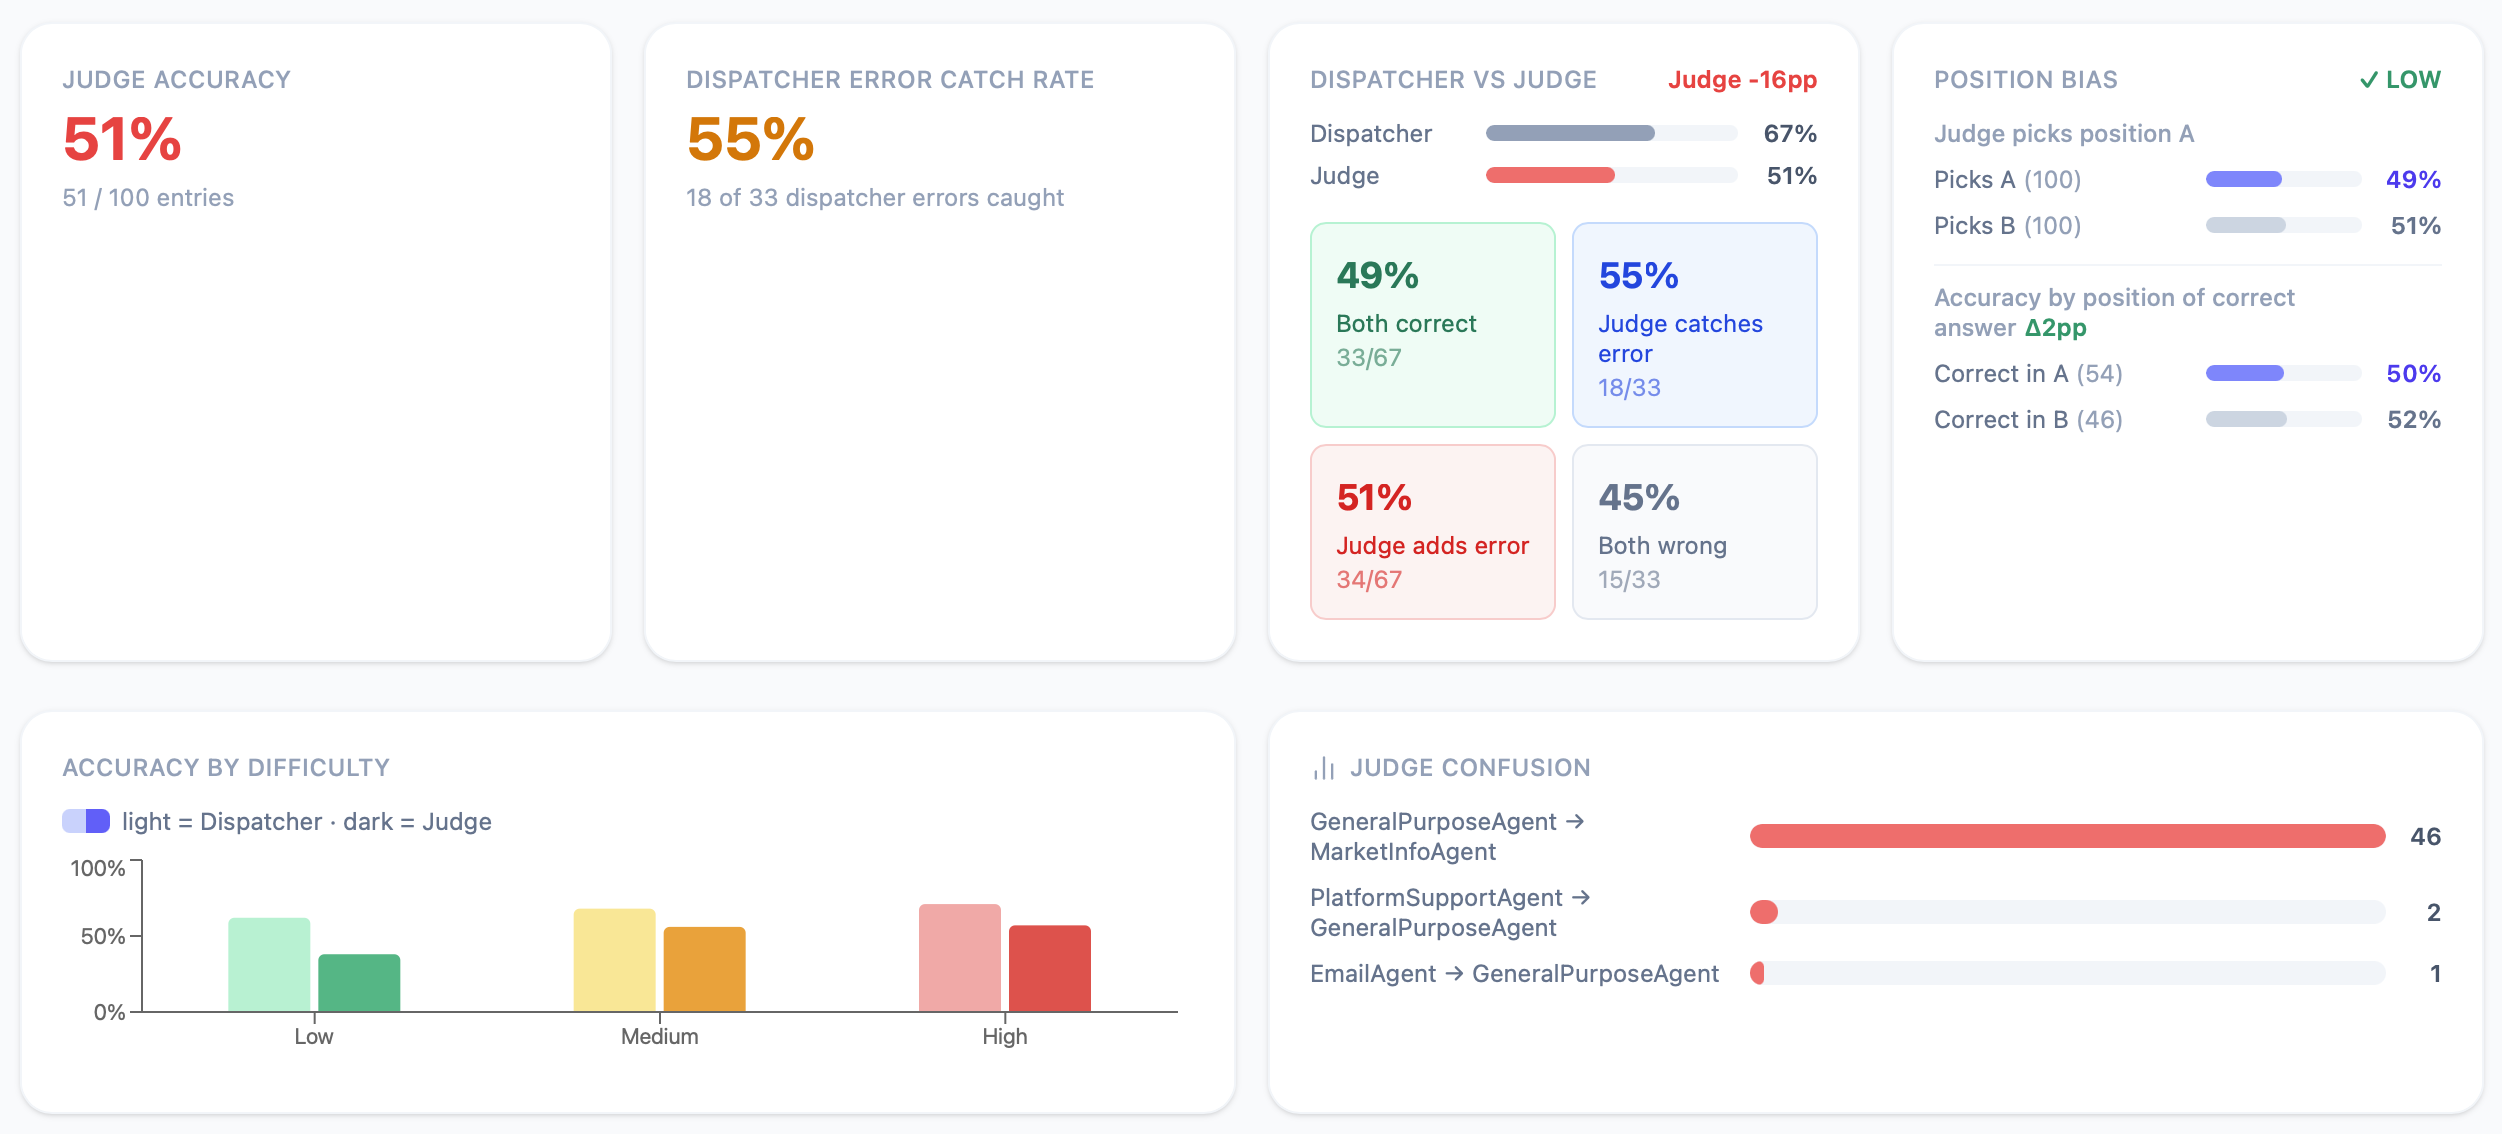
\includegraphics[keepaspectratio]{assets/pipeline/fig3_dashboard_basic_prompt.png}}
\caption{Judge evaluation on the training dataset using Gemma4 31b and a basic comparison prompt.}
\label{fig:judge-basic-prompt}
\end{figure}


The dashboard shows a position distribution close to even, with no indication of a position bias. This finding does not make the mitigation unnecessary. A systematic study by \textcite{shi2024positionbias} confirms that the direction and strength of the position bias vary across judge models and tasks, so the safeguard remains relevant for future model changes.

The results show a judge agreement of 51\% with the ground truth dataset, which is rarely better than chance for a binary decision. The confusion metric revealed a recurring pattern. The judge systematically preferred MarketInfoAgent responses over those from the GeneralPurposeAgent, even when the router had correctly selected the latter. Inspecting these cases showed that MarketInfoAgent responses were consistently more verbose and included comparison tables, section headers, and a data limitation note, while GeneralPurposeAgent responses tend to be shorter and less structured. The judge interpreted these formatting features as signals of quality rather than style. This is an appearance of style bias, which \textcite{soumik2026biasmitigation} identifies as the dominant bias among LLM judges, compounded by verbosity bias, the tendency to favor longer answers regardless of their actual content \autocite{zheng2023judging}.

Style bias is mitigated through evaluation rubrics, which is a set of explicit, structured criteria the judge applies for its evaluation instead of unconstrainedly performing an overall judgement. The results reported by \textcite{kim2024prometheus} show that fine-grained rubrics let smaller models reach the agreement levels of much larger ones without such rubrics.

The judge's rubric consists of three routing-specific criteria that are the result of iterative testing until the best results were reached. Helpfulness assesses how well the response resolves the broker's actual request. Specificity assesses whether the response reflects the domain knowledge of the appropriate specialized agent and stays within the scope of the query. Conciseness assesses whether the response is as direct as the query requires. The judge is prompted to apply these criteria sequentially rather than all at once. It first produces a short comparative assessment per criterion, evaluating both candidates on one criterion before moving to the next, and only then forms its final verdict and justification. This sequencing follows the chain-of-thought, form-filling approach introduced by \textcite{liu2023geval} for LLM-based evaluation, and makes it harder for a single feature, such as a table, to dominate the outcome.

\begin{figure}
\centering
\pandocbounded{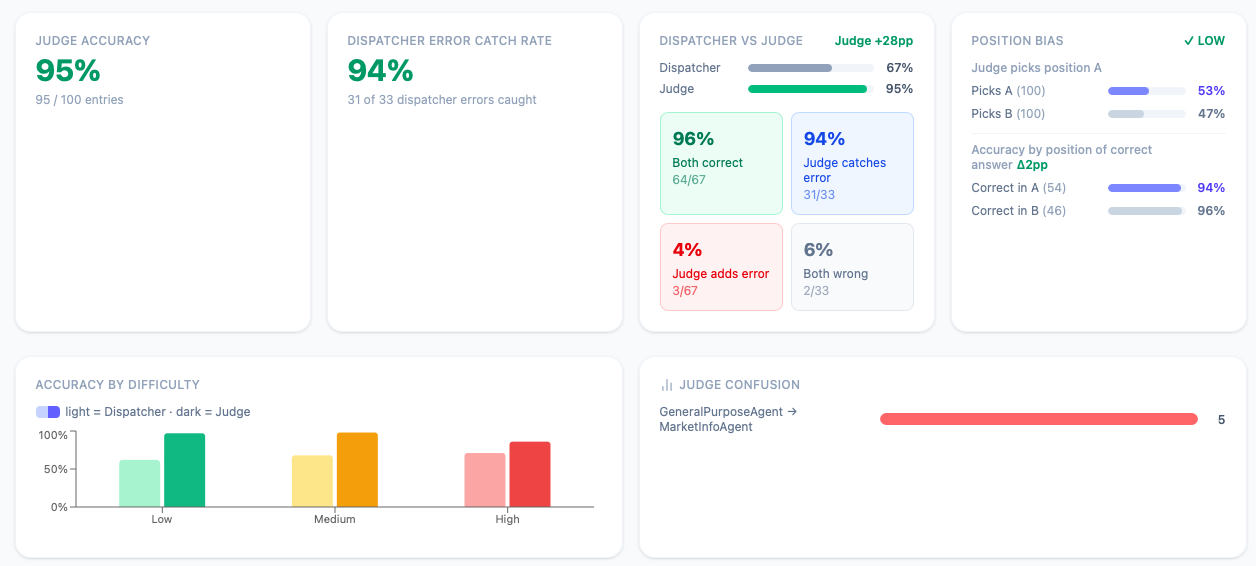
\includegraphics[keepaspectratio]{assets/pipeline/fig4_dashboard_rubrics.png}}
\caption{Judge evaluation on the training dataset using Gemma 4 31b and routing-specific rubrics.}
\label{fig:judge-rubrics}
\end{figure}


Introducing rubrics raised the judge accuracy by 44 percentage points on the dataset with the 100 most uncertain queries (\cref{fig:judge-rubrics}). Once the team gathered access to AWS Bedrock, the judge model was migrated to Claude Sonnet 4.6 and evaluated on the 1,000-query golden dataset to ensure it generalizes on unseen queries.

\begin{figure}
\centering
\pandocbounded{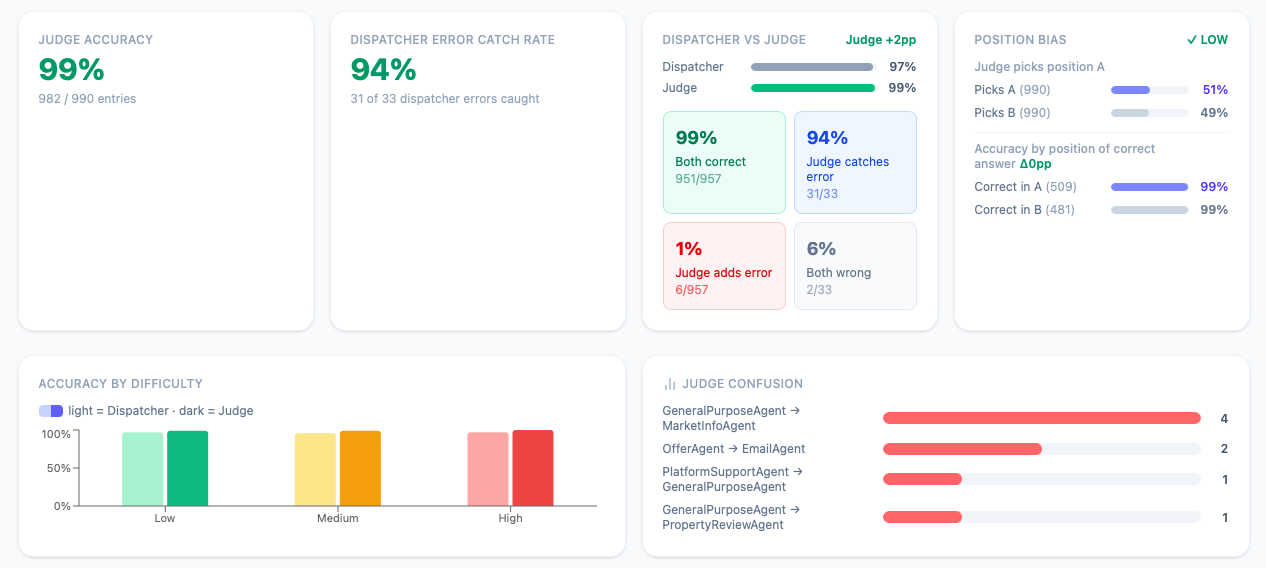
\includegraphics[keepaspectratio]{assets/pipeline/fig5_dashboard_sonnet.png}}
\caption{Judge evaluation on the evaluation dataset using Claude Sonnet 4.6 and routing-specific rubrics.}
\label{fig:judge-sonnet}
\end{figure}


The final evaluation reached 99\% agreement (\cref{fig:judge-sonnet}), confirming the judge is reliable enough to grade the router's decisions. In the evaluation, 10 out of the 1,000 queries were excluded due to API overload during the agent response generation, leading to empty responses returned by the agents.

Another recognized strategy against individual judge biases is replacing the single judge with a panel of models that aggregate their verdicts \autocite{verga2024juries}. Survey work classifies such multi-judge setups among the established mitigation strategies \autocite{gu2024llmjudge}. The option was rejected for this project for multiple reasons. First, costs scale linearly with the panel size, which is the dominant factor for a component running on every query. Second, the benefit of a panel supposes diverse model families, since judges from the same family share the same biases, and aggregation then reinforces these biases rather than cancelling them. A credible cross-family panel was not available within the project's LLM access constraints. Third, each panel member would also require its own prompt engineering and validation, which multiplies the iteration effort documented above beyond what the project's timeline allowed. Given that the single-judge setup already reached 99\% agreement, a panel remains an option in the future only if the judge accuracy drops on newly constructed test queries.

\subsubsection{Implementation}\label{sec:judge-implementation}

The previous sections described how the judge reaches its verdict. This section focuses on the implementation of the judge module from a processual perspective. It describes which steps are taken within the judge module and how the judge verdict flows back into the router's two stages to correct routing decisions and improve future performance. \Cref{fig:judge-process} illustrates the three cases that govern this process.

\begin{figure}
\centering
\pandocbounded{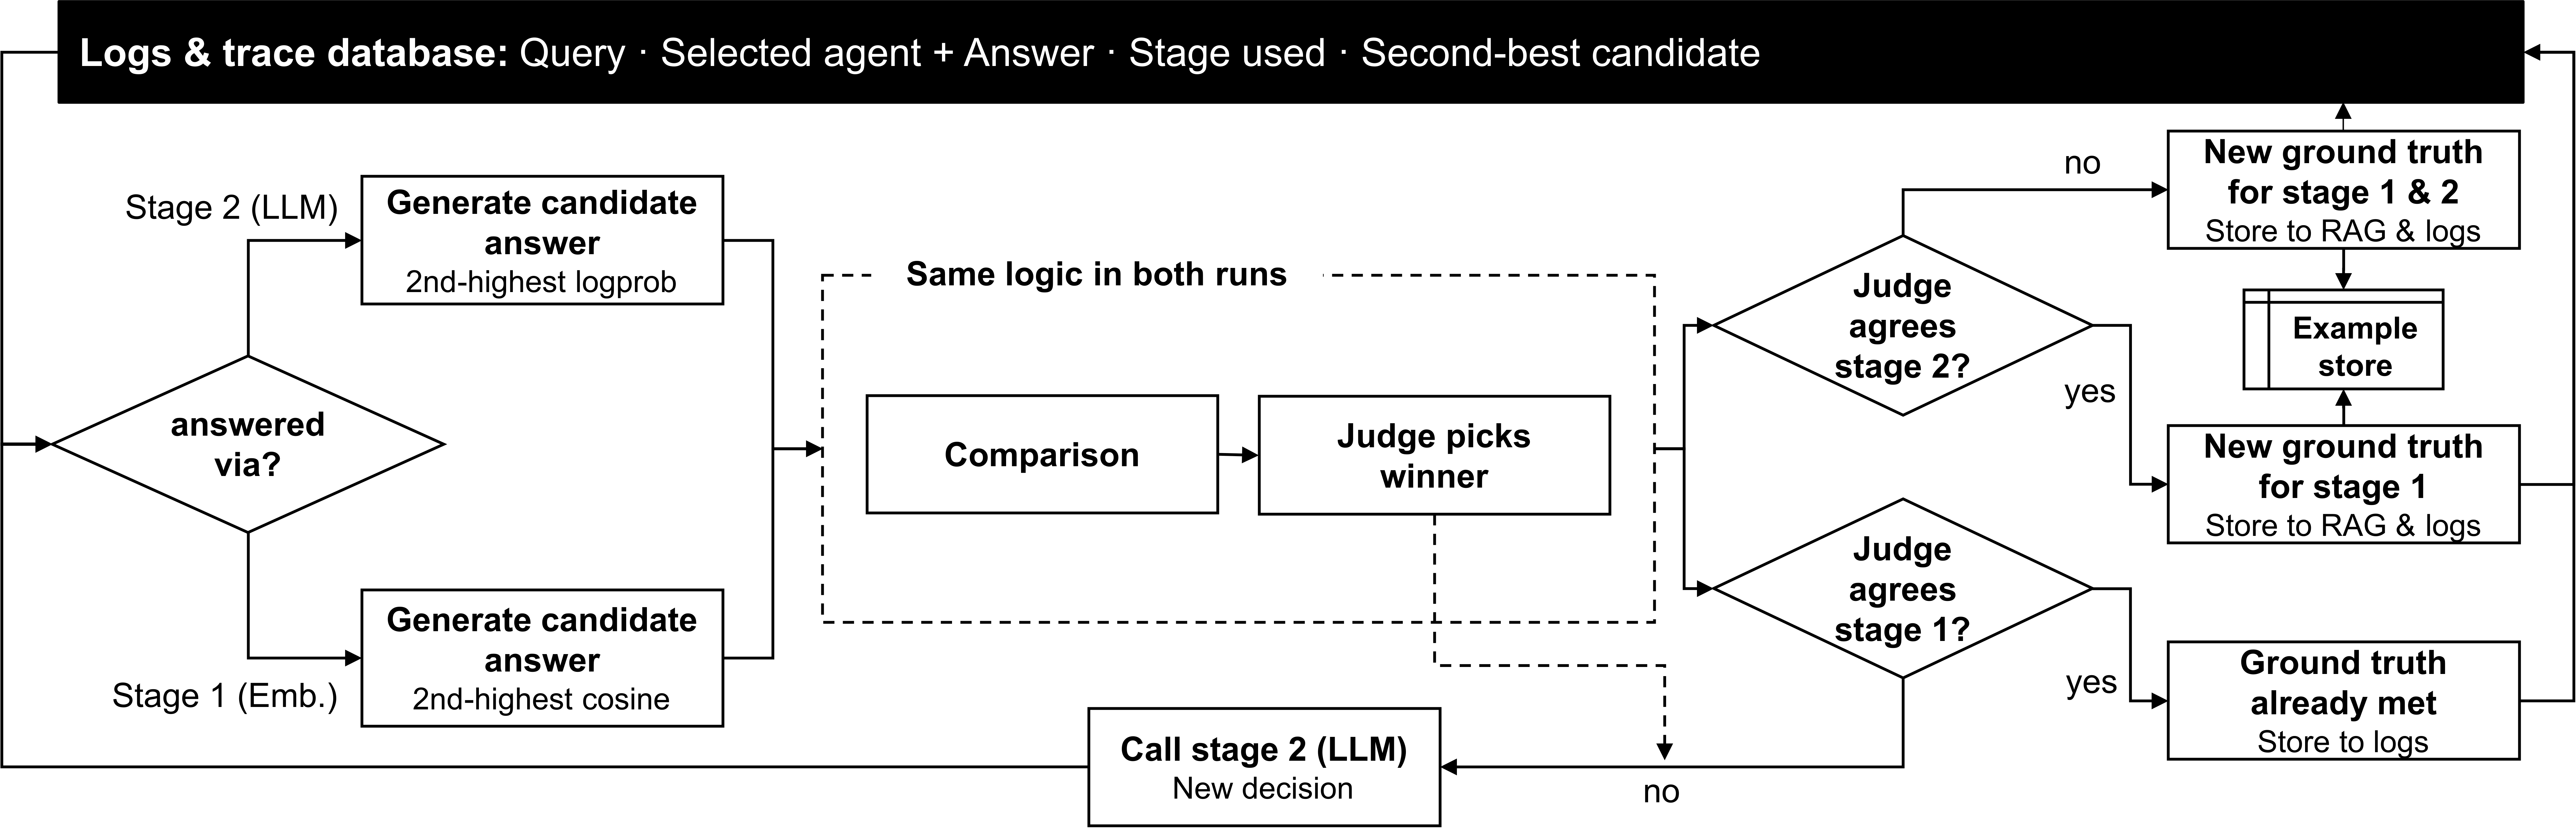
\includegraphics[keepaspectratio]{assets/pipeline/judge-process.png}}
\caption{Process Diagram of the Judge module with Stage 1 correction mechanism and storage of signals for the optimizer.}
\label{fig:judge-process}
\end{figure}


Within the judge module, several distinctions are made when a new query to be evaluated is consumed from the router's logs. First, a check is performed which Stage of the router performed the routing decision. If Stage 1 routed the query and the judge agrees, no correction is written, as Stage 1 is already correct. If Stage 1 routed the query and the judge disagrees, the query is escalated to Stage 2, which identifies its own top two candidates. Since these can differ from Stage 1's choices, Stage 1's original winner is carried into this second evaluation alongside the Stage 2 candidates, so the judge compares all three together rather than only the two Stage 2 proposed. This ensures that in ambiguous cases where Stage 1 and Stage 2 choose different agent pairs, the judge considers a broader scope of potential agents for the evaluation. If the query was initially already routed via Stage 2, this indicates that Stage 1 was too uncertain to decide at all, as no agent-specific threshold was met. In this case the judge evaluates Stage 2's decision directly and writes the query and the winning agent back to the example store of Stage 1.

In short, Stage 1 is corrected whenever it was wrong or too uncertain to decide, while the optimizer receives a signal whenever Stage 2 itself was judged incorrect. A novelty check blocks entries whose cosine similarity to an existing example exceeds 0.96, preventing redundant duplicates. Over time, this write-back extends the range of queries that Stage 1 resolves directly, which reduces the number of escalations to Stage 2 of the router and with that the cost and latency, while improving accuracy.
